
\section{Particles in the heliosphere}

\begin{figure}
	\centering
	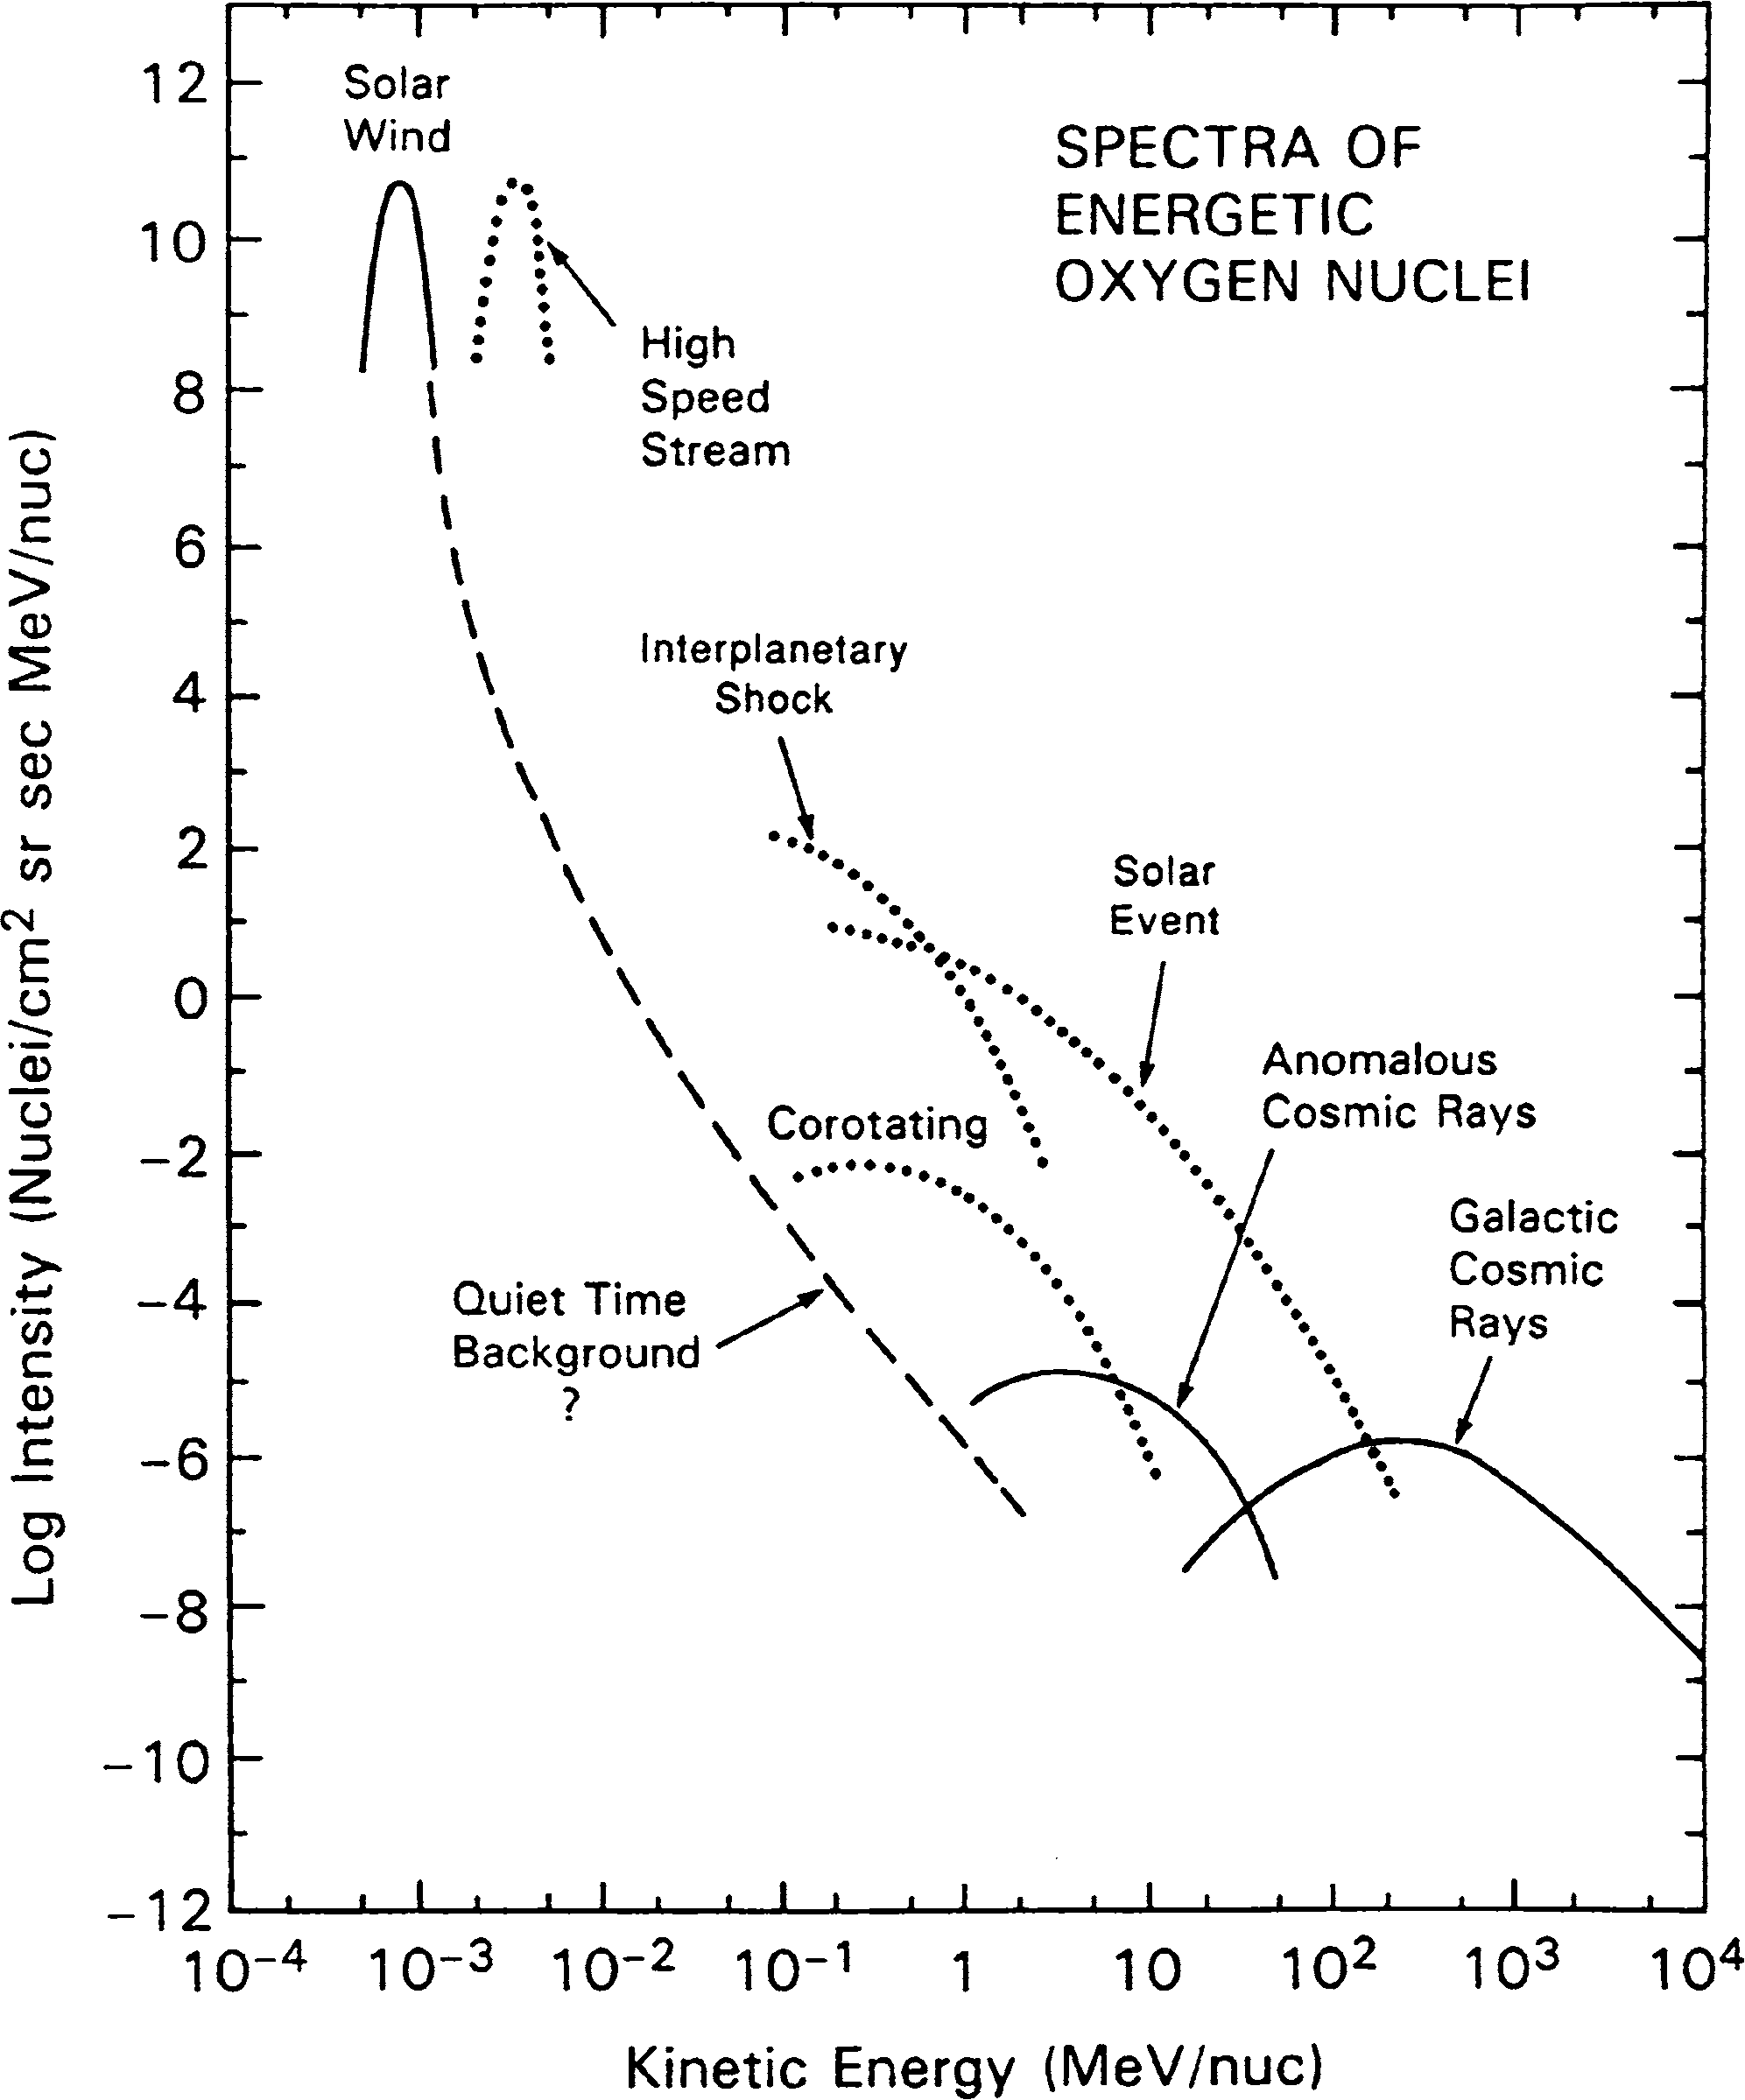
\includegraphics[width=0.6\linewidth]{images/heliospheric_energy_spectrum}
	\caption[Spectra of oxygen ions in the near-Earth interplanetary space]{Typical spectra of oxygen ions in the near-Earth interplanetary space, showing the contributions from different populations. Other particle species show similarly shaped spectra when plotted as a function of energy/nucleon. (adapted from \url{http://helios.gsfc.nasa.gov/ace/gallery.html}).}
	\label{fig:heliospheric_energy_spectrum}
\end{figure}

\section{Coronal mass ejections}

\section{Forbush decreases}

\section{Motivation}

\ac{MSL}/\ac{RAD}